

\documentclass[a4paper]{article}

\usepackage{amsmath}
\usepackage{hyperref}
\usepackage{biblatex}
\usepackage{enumerate}
\usepackage{graphicx}
\usepackage{stmaryrd}
\usepackage[dvipsnames]{xcolor}
\usepackage{listings}
\usepackage{caption}
\usepackage{subcaption}
\usepackage{booktabs}


\addbibresource{refs.bib}

\begin{document}

\author{Ola Bratt \\
  \href{mailto:ola.bratt@gmail.com}{ola.bratt@gmail.com}
  \and
  Patrick Attimont \\
  \href{patrickattimont@gmail.com}{patrickattimont@gmail.com}
}

\title{DAT565/DIT407 Assignment 4}
\date{2024-02-xx}

\maketitle

This paper is addressing the assignment 3 study queries within the \emph{Introduction to Data Science \& AI} course, DIT407 at 
the University of Gothenburg and DAT565 at Chalmers. The main source of information for this project
is derived from the lectures and Skiena~\cite{Skiena:2024}. Assignment 4 is about correlation and linear regression.

\section*{Problem 1: Splitting the data}
The dataset is large enough to be separated into a train and a test set. We use the function \verb|train_test_split| with a test size of 0.2.


\section*{Problem 2: Single-variable model}
To identify the variable with the strongest linear relationship with the target variable, we use the \verb|corr| function specifying the Pearson method to get a correlation matrix between all the variables, and take the column corresponding to the target variable.

The variable with the highest absolute pearson coefficient is the Human development index, with a value of 0.92.
Fig~\ref{fig:reg_human_development_index} shows the linear regression applied on the test set, using the model built on the train set.
The model has a slope of 48.2, an intercept of 37.3, and a determination coefficient of 0.86. These values obviously slightly change depending on the seed used to split the data.
The mean squared error for is 9.45.


\begin{figure}[h]
  \begin{center}
    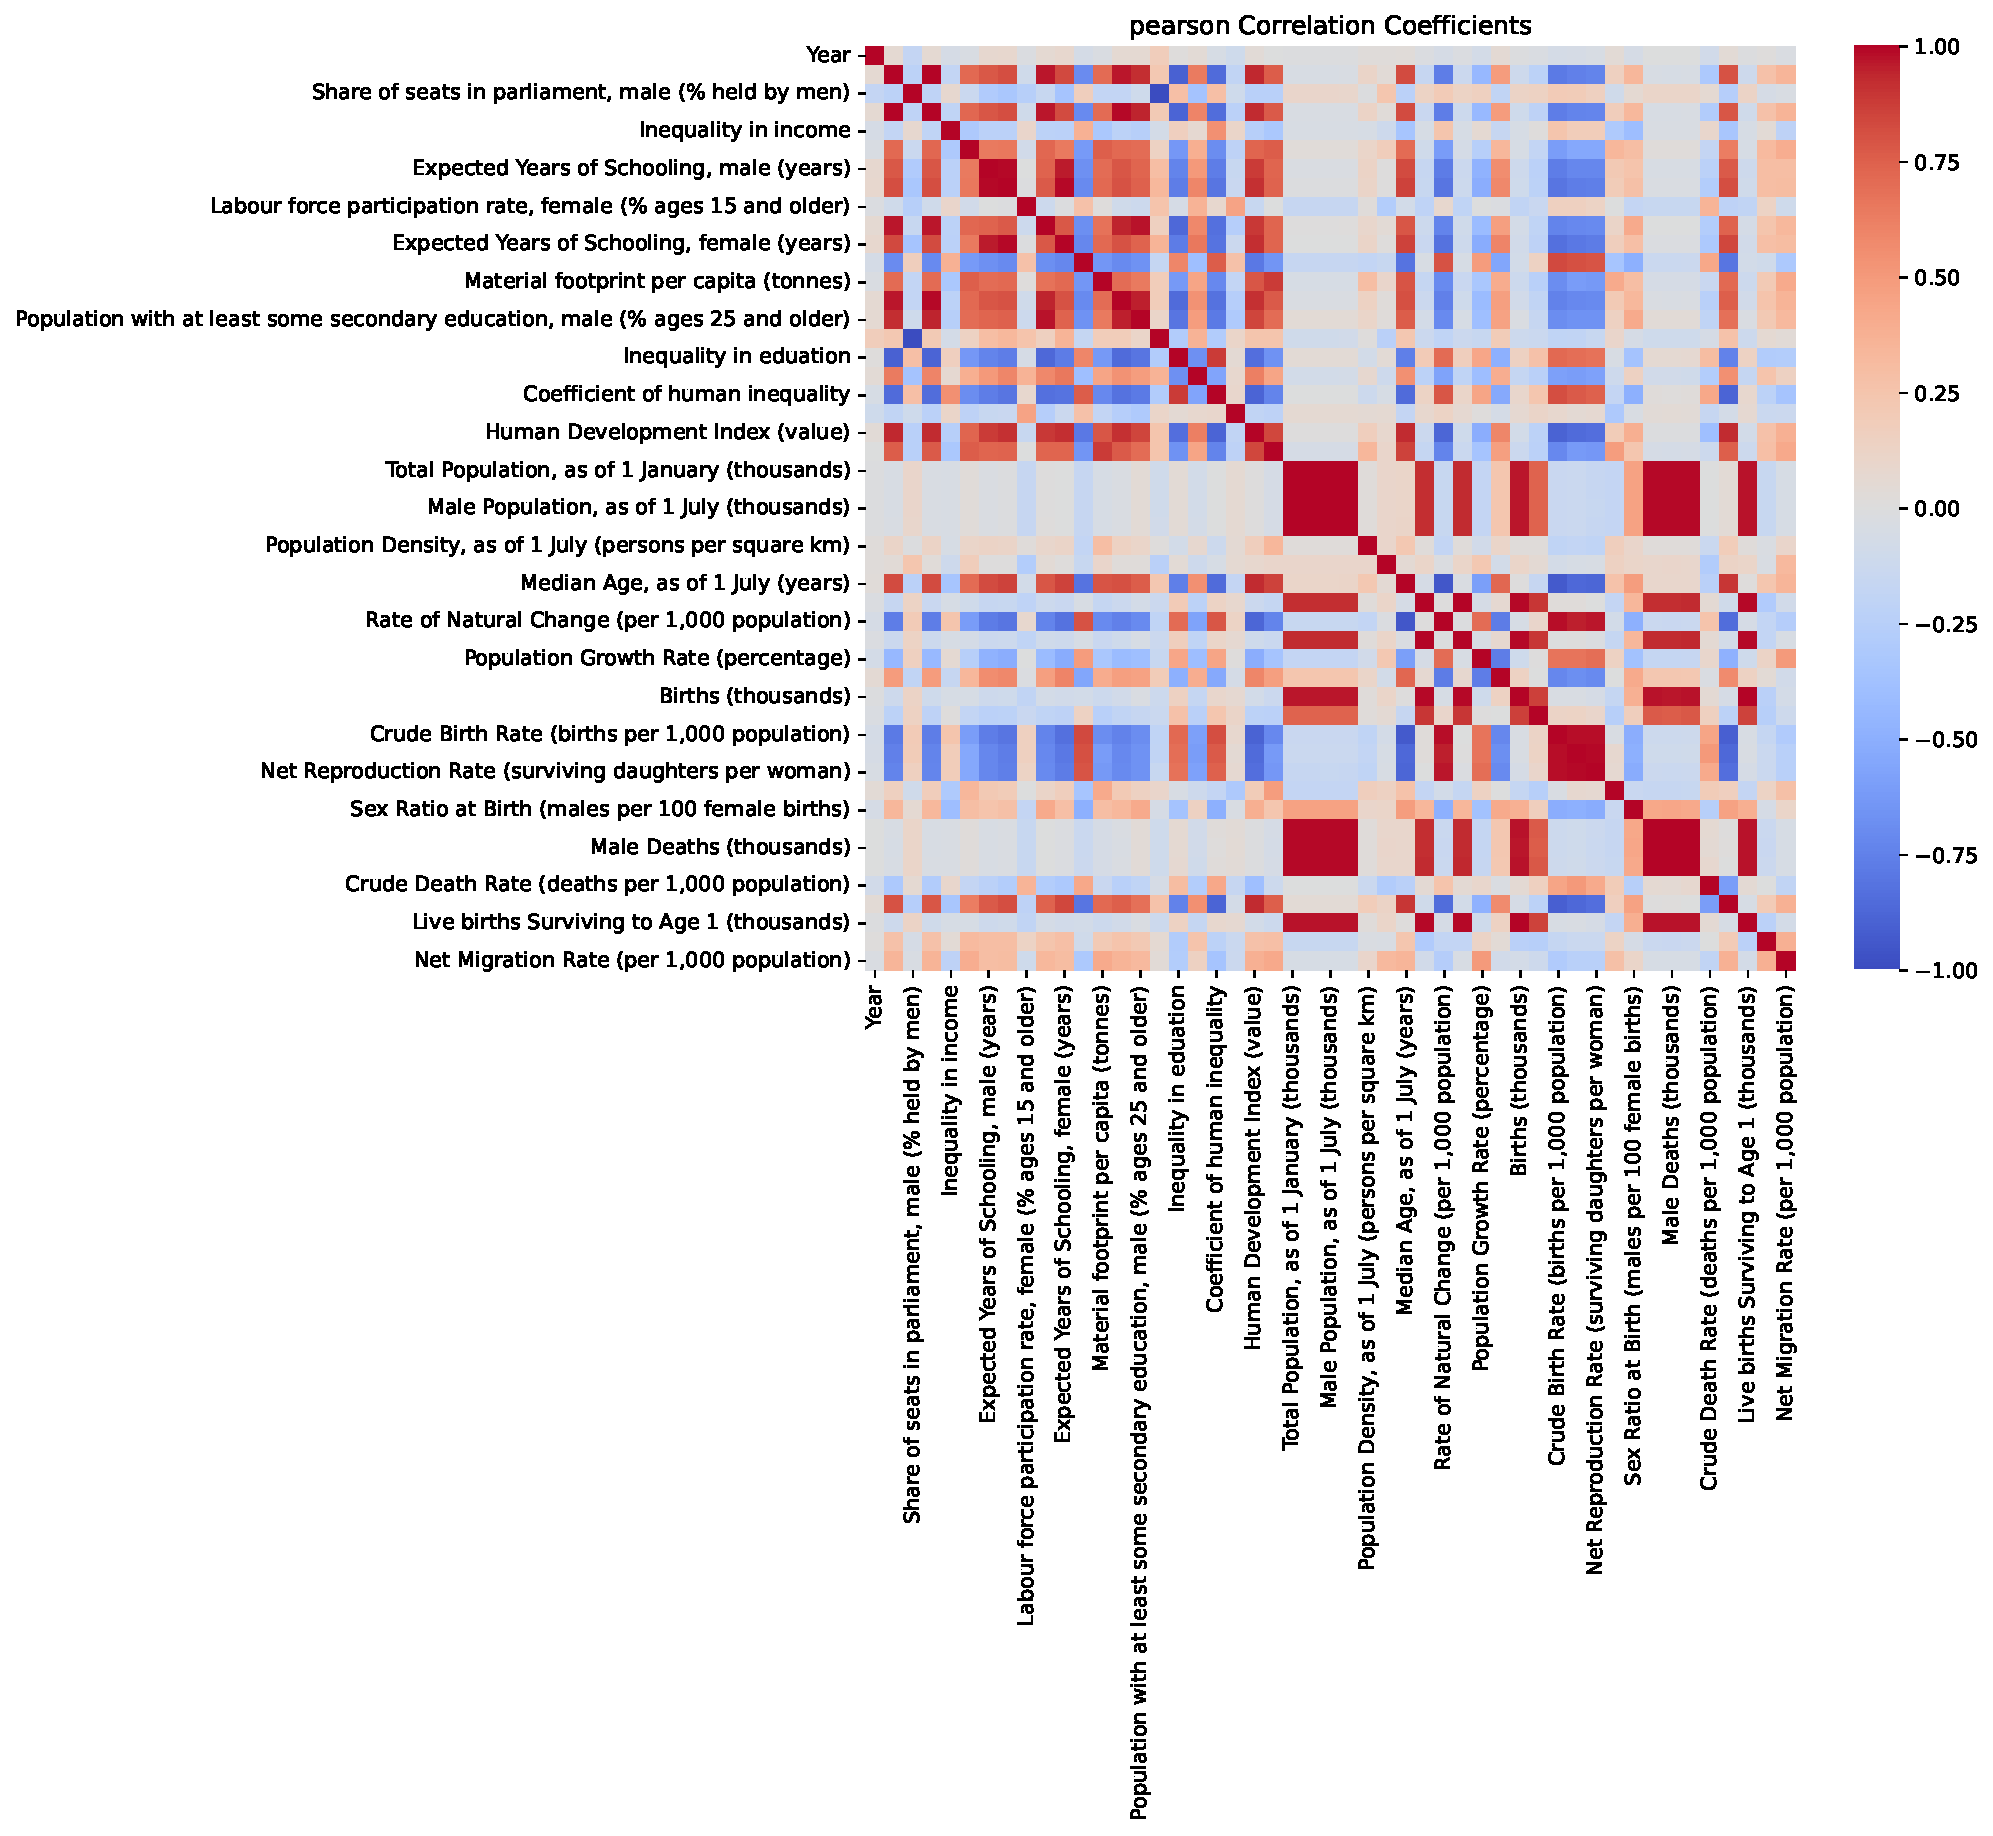
\includegraphics[width=\textwidth]{ola/pearson_correlation.pdf}
    \caption{Correlation Pearson}
    \label{fig:pearson_correlation}
  \end{center}
\end{figure}

\begin{figure}[h]
  \begin{center}
    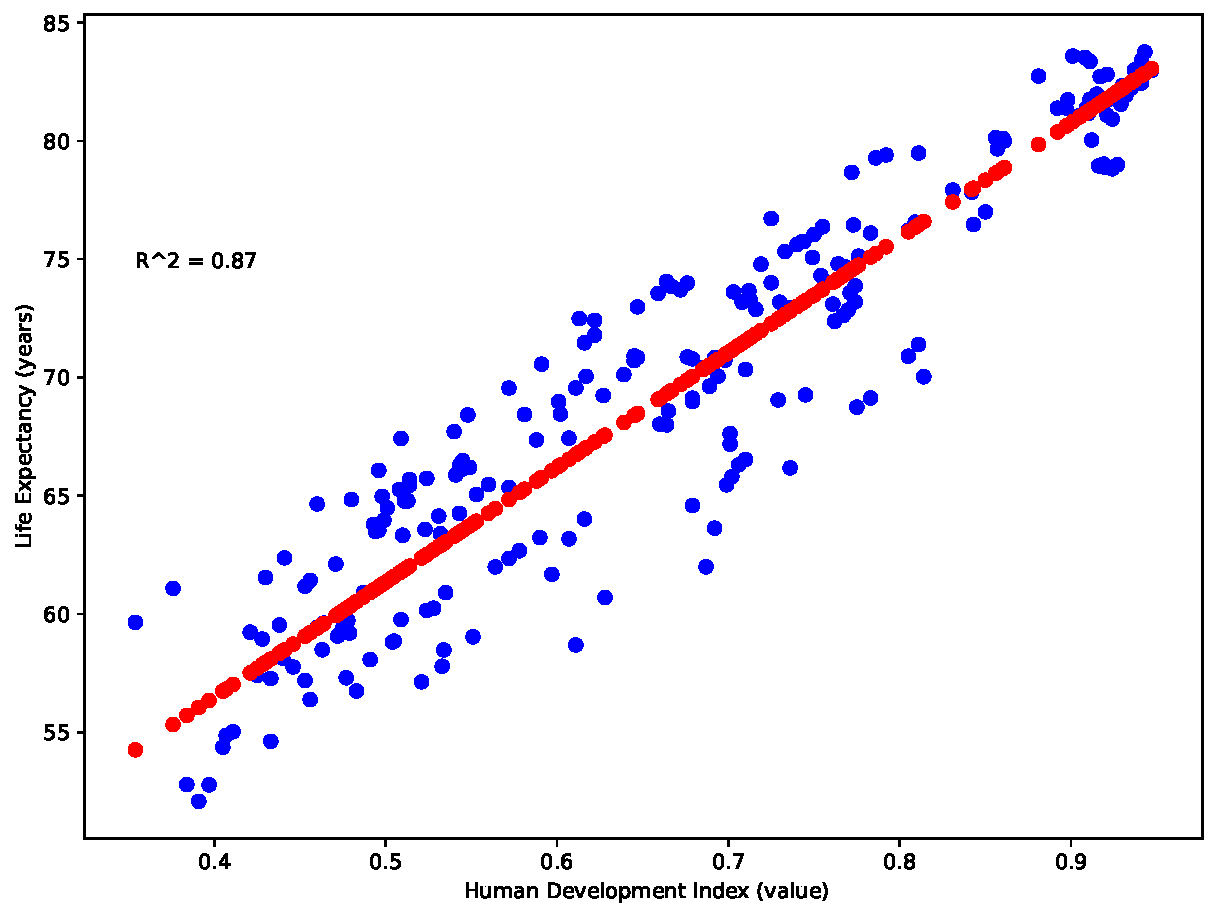
\includegraphics[width=\textwidth]{ola/_linear_regression_human_development_index_(value).pdf}
    \caption{Linear Regression Human Development Index (value)}
    \label{fig:reg_human_development_index}
  \end{center}
\end{figure}

\section*{Problem 3: Non-linear relationship}

To explore variables with non-linear relationships, we initially assess Spearman correlation coefficients, Figure~\ref{fig:spearman_correlation}. 
Initially, we eliminate the variable exhibiting the strongest Pearson correlation, namely 'Human Development Index (value)'. Subsequently, we examine the Spearman correlation.

Our analysis reveals that 'Median Age, as of 1 July (years)' exhibits the most robust Spearman correlation. Subsequently, 
we develop a linear model using this variable to determine the mean squared error, which amounts to 13.58, Figure~\ref{fig:reg_median_age}.

Next, we apply transformations to the variable using logarithmic, square root, and reciprocal functions, respectively  Figure~\ref{fig:linear_transformation}. 
For each transformation, we train a linear model to ascertain the resulting mean squared error. The logarithmic transformation yields the lowest mean squared error, measuring 11.52.  Figure~\ref{fig:reg_median_age_log}.

Before transformation, the Pearson correlation registers at 0.898, while after transformation, it increases marginally to 0.913.


\begin{figure}[h]
  \begin{center}
    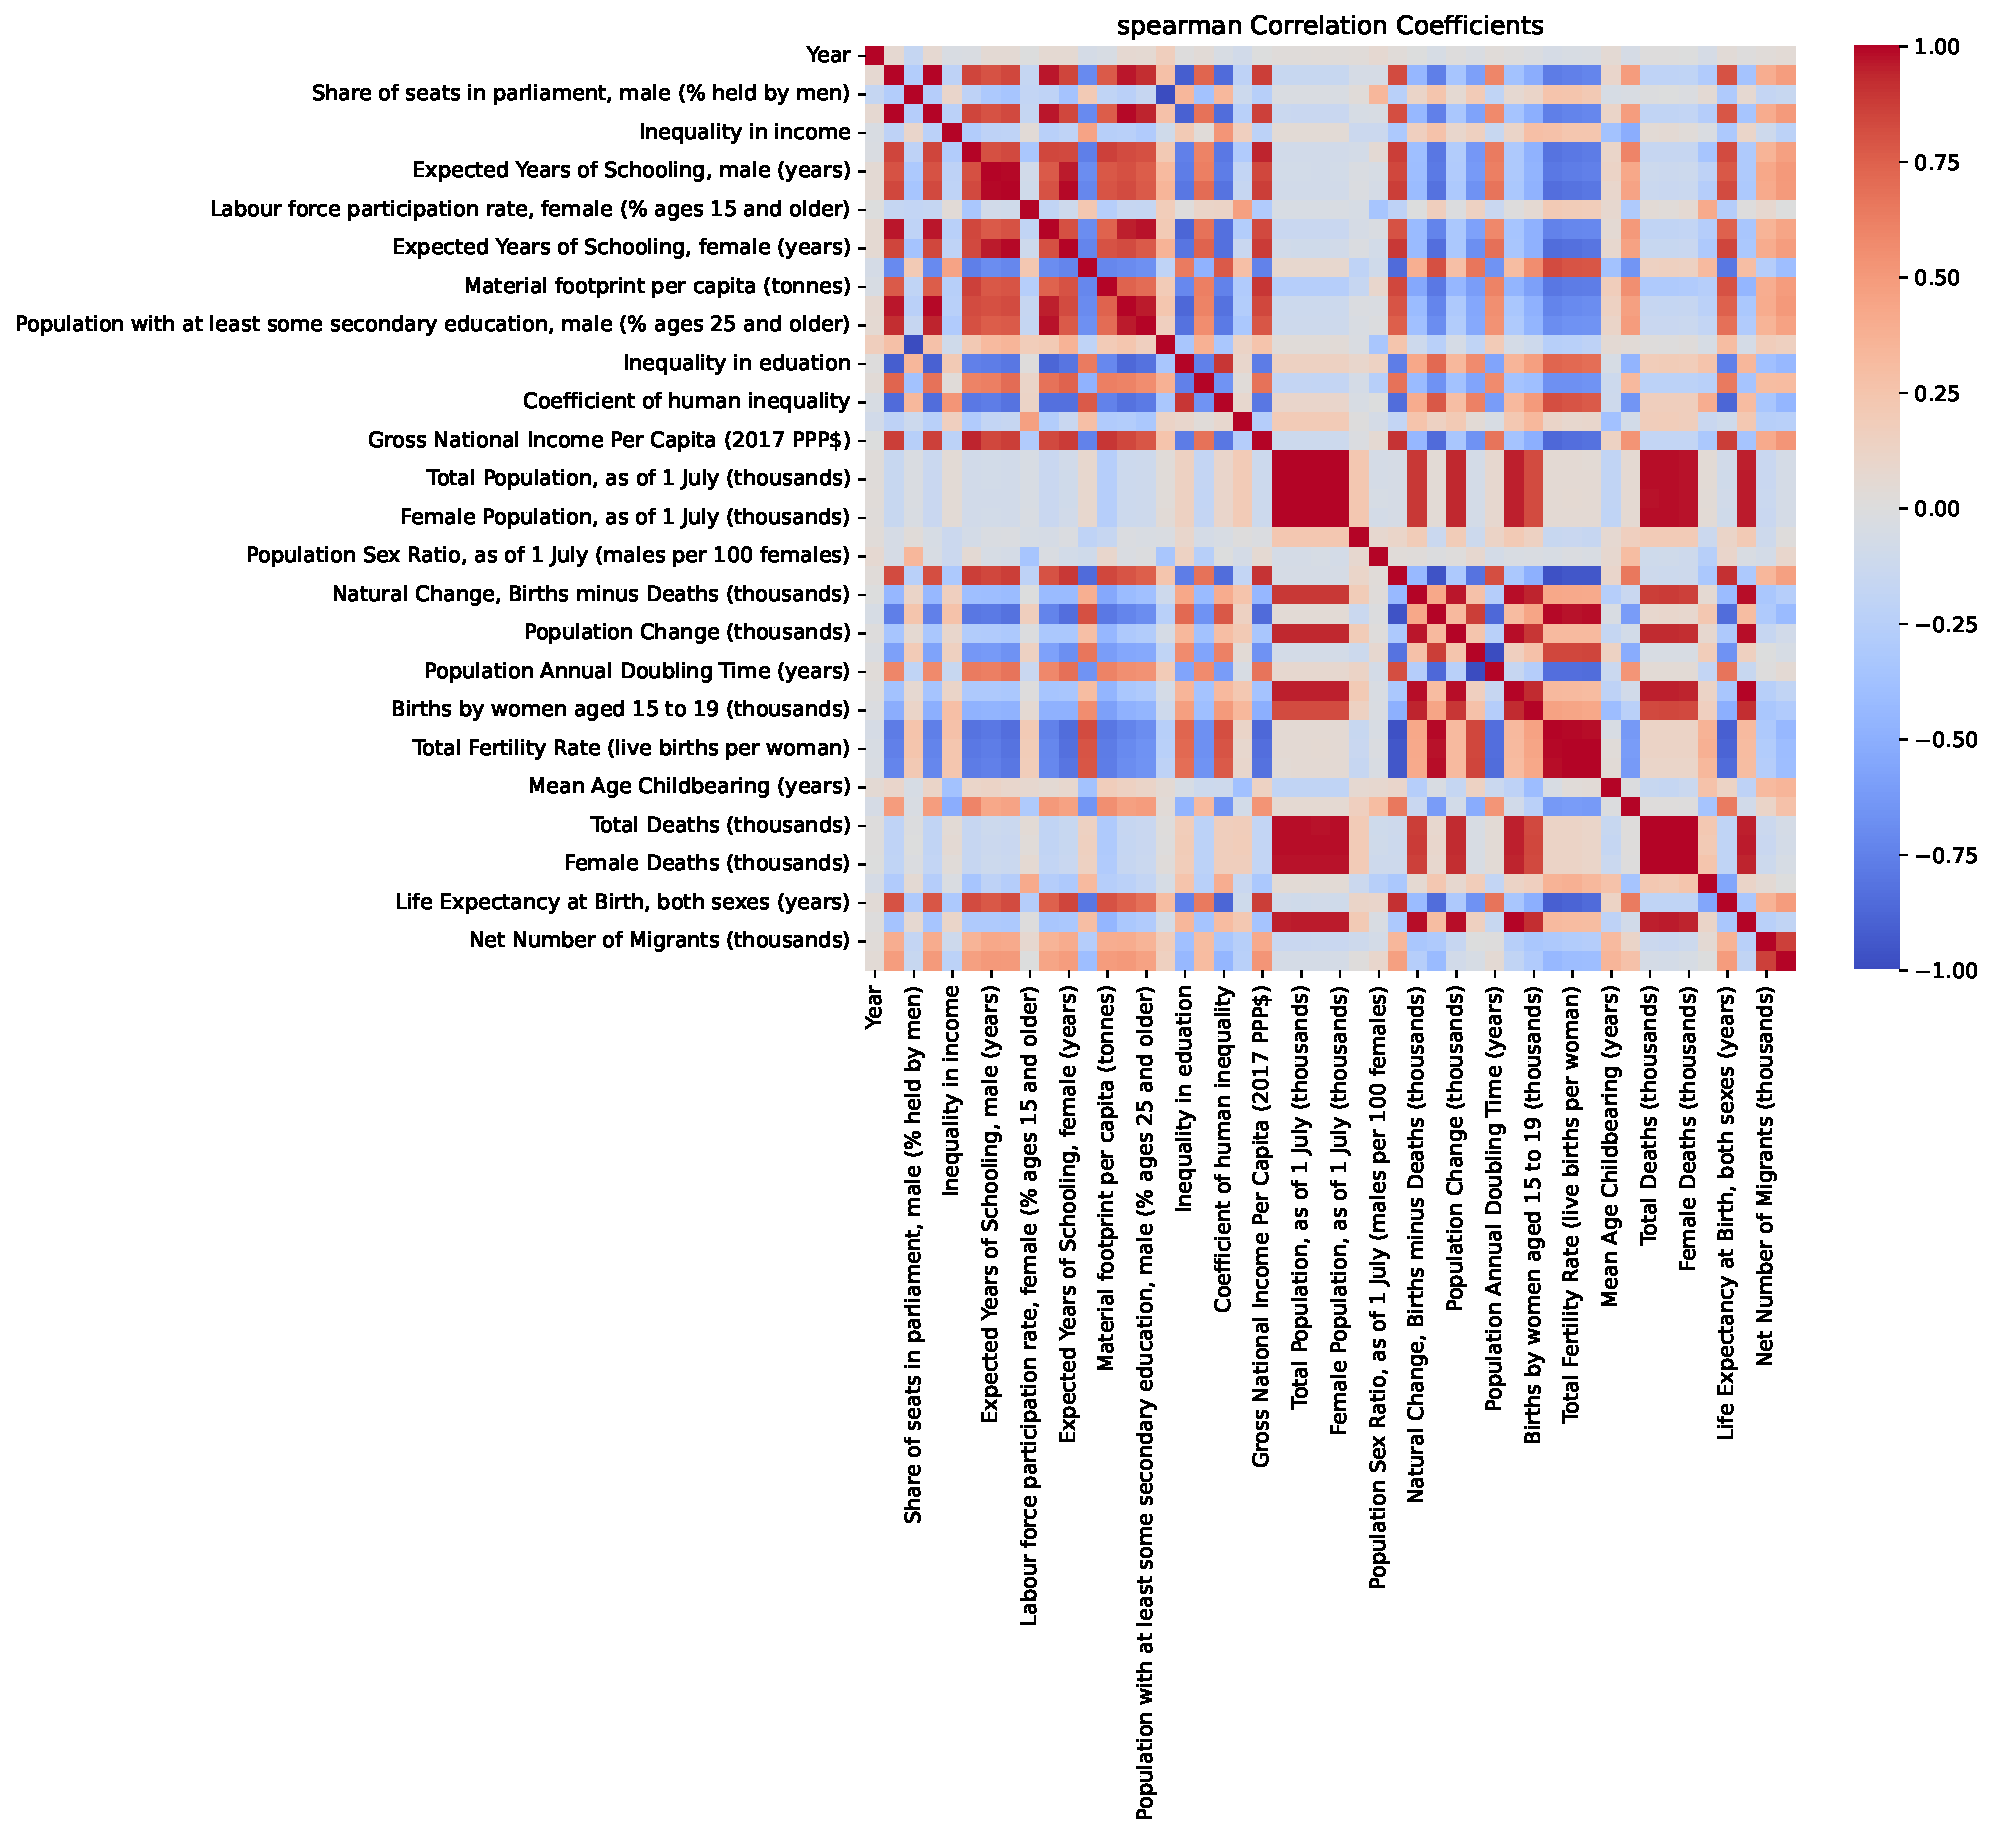
\includegraphics[width=\textwidth]{ola/spearman_correlation.pdf}
    \caption{Correlation Spearman}
    \label{fig:spearman_correlation}
  \end{center}
\end{figure}


\begin{figure}[h]
  \begin{center}
    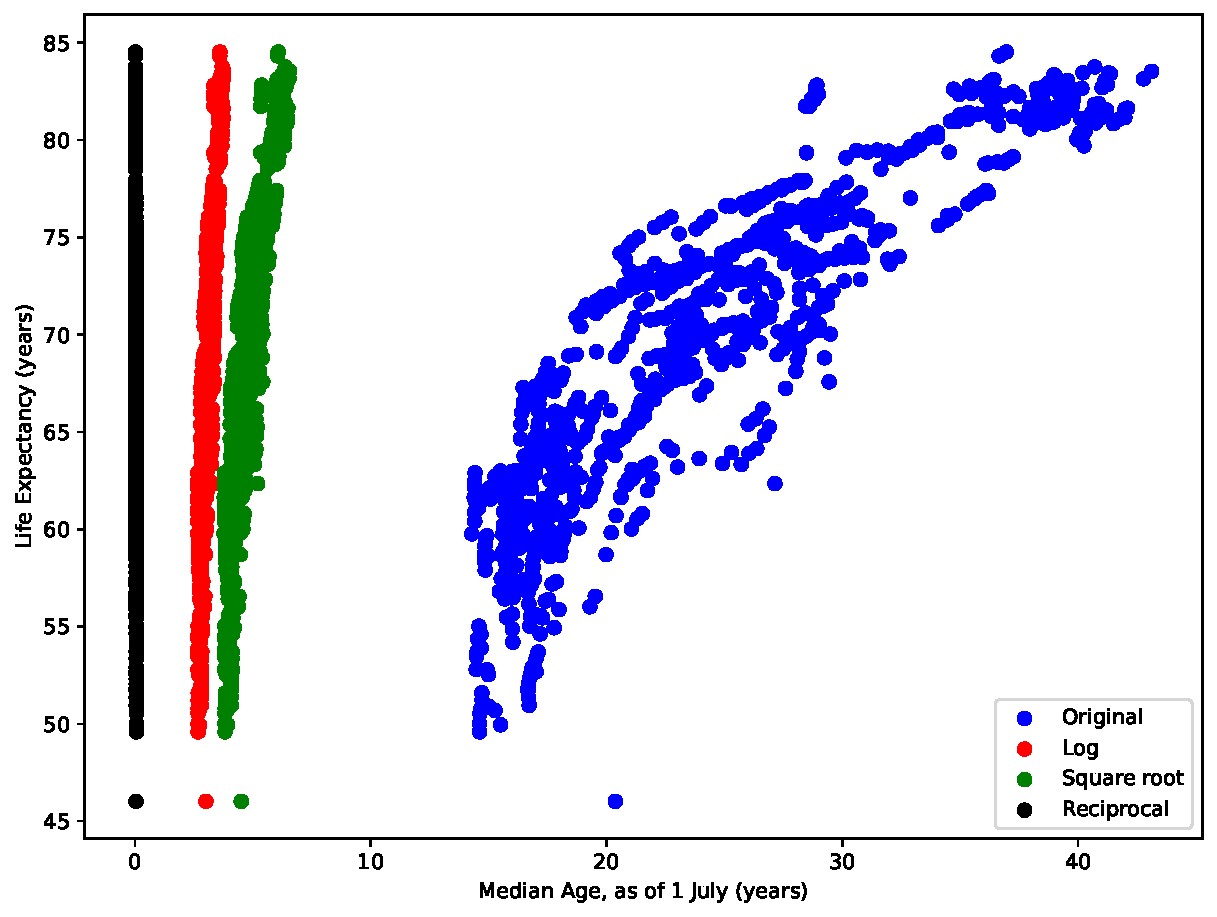
\includegraphics[width=\textwidth]{ola/linear_transformation.pdf}
    \caption{Linear transformation}
    \label{fig:linear_transformation}
  \end{center}
\end{figure}

\begin{figure}
  \centering
  \begin{subfigure}[a]{\textwidth}
      \centering
      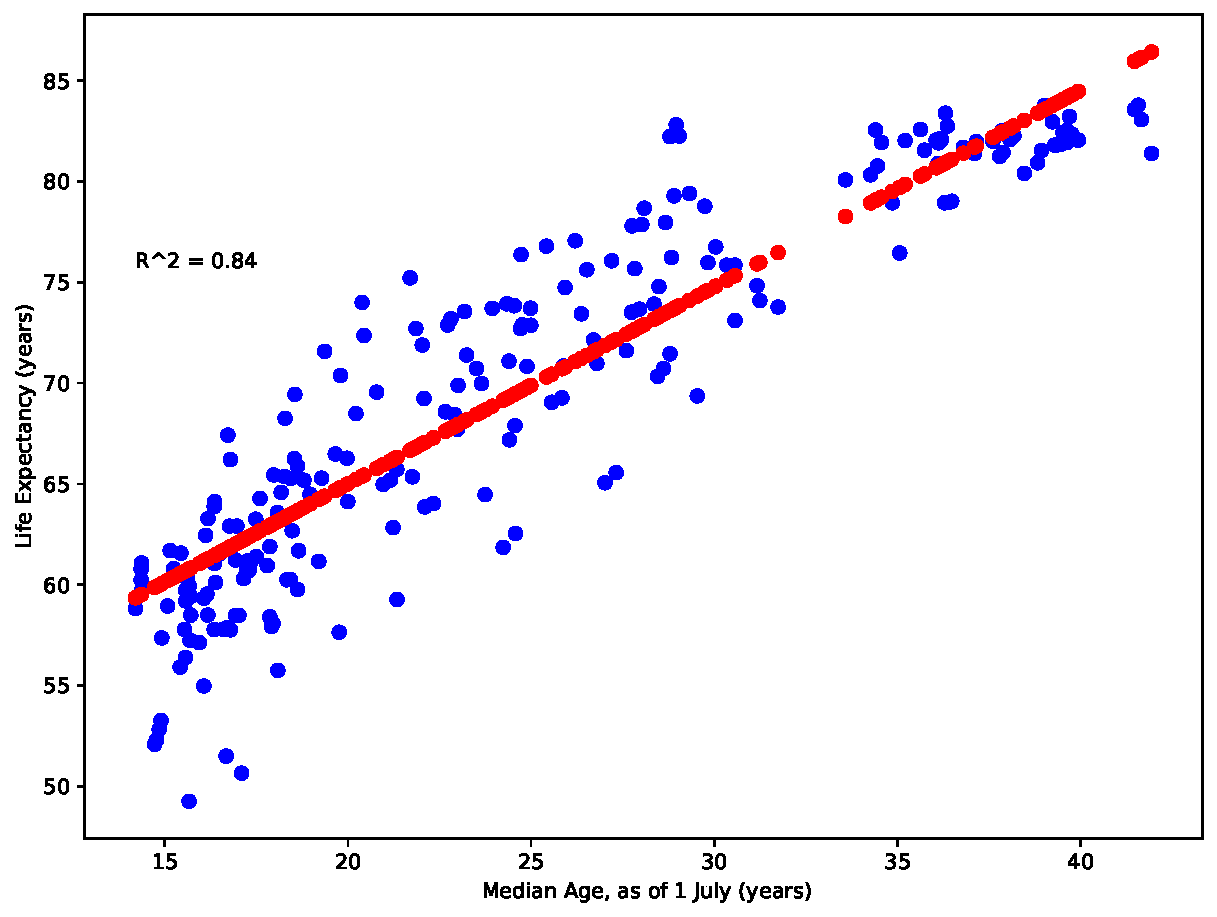
\includegraphics[width=\textwidth]{ola/_linear_regression_median_age,_as_of_1_july_(years).pdf}
      \caption{Linear Regression Median Age (original)}
      \label{fig:reg_median_age}
  \end{subfigure}
  \vfill
  \begin{subfigure}[b]{\textwidth}
      \centering
      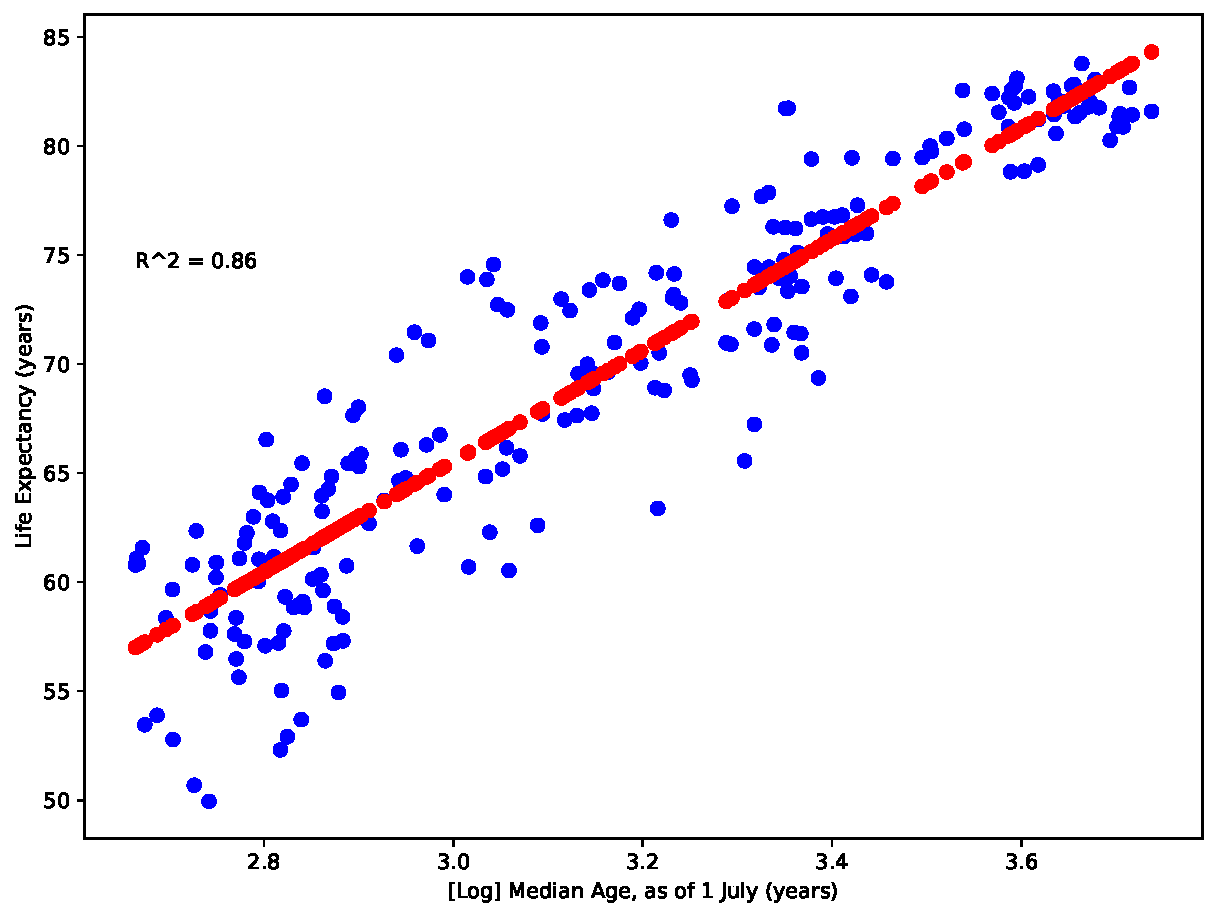
\includegraphics[width=\textwidth]{ola/[log]_linear_regression_median_age,_as_of_1_july_(years).pdf}
      \caption{Linear Regression Median Age (log)}
      \label{fig:reg_median_age_log}
  \end{subfigure}
  \caption{Linear Regression Median Age}
  \label{fig:linear_regression_median_age}
\end{figure}

\section*{Problem 4: Mulitple linear regression}

We employ Spearman correlation analysis to identify variables with strong correlations. Utilizing a predefined threshold, we pinpoint variables with significant impact. 
Through experimentation with various thresholds, we determine that a threshold of 0.85 yields favorable results without excessive variable inclusion.

The identified variables include: Expected Years of Schooling, female (years), Coefficient of human inequality, Gross National Income Per Capita (2017), Median Age as of 1 July (years), Rate of Natural Change (per 1,000 population), Crude Birth Rate (births per 1,000 population), Total Fertility Rate (live births per woman), and Net Reproduction Rate (surviving daughters per woman).

Conducting a multiple linear regression analysis results in a mean squared error of 2.03. The coefficients for the model are as follows: [19, -571, 243338, 61, 1.7, -2.1, 1.9, 3].




\newpage


\printbibliography

\section*{Appendix: Source Code}

\lstset{
  language=Python,
  basicstyle=\ttfamily,
  commentstyle=\color{OliveGreen},
  keywordstyle=\bfseries\color{Magenta},
  stringstyle=\color{YellowOrange},
  numbers=left,
  basicstyle=\footnotesize,
  breaklines=true,
  postbreak=\mbox{\textcolor{red}{$\hookrightarrow$}\space}
}


\lstinputlisting{ola/assignment4.py}

\end{document}
